\documentclass{beamer}
\usetheme[numbering=fullbar]{focus}
\setbeamertemplate{mini frames}{}
\usepackage[labelformat=simple]{subfig}
\usepackage{graphicx}
\usepackage[export]{adjustbox}
\usepackage[version=4]{mhchem}
\usepackage{fix-cm}
\usepackage{multicol}
\usepackage{mathtools}
\renewcommand{\thesubfigure}{\relax}

\title{CG Method Comparison \\ for a FEM IMEX Scheme}
\subtitle{Math 693A Final Project Presentation}
\author{Geneva Porter}
\titlegraphic{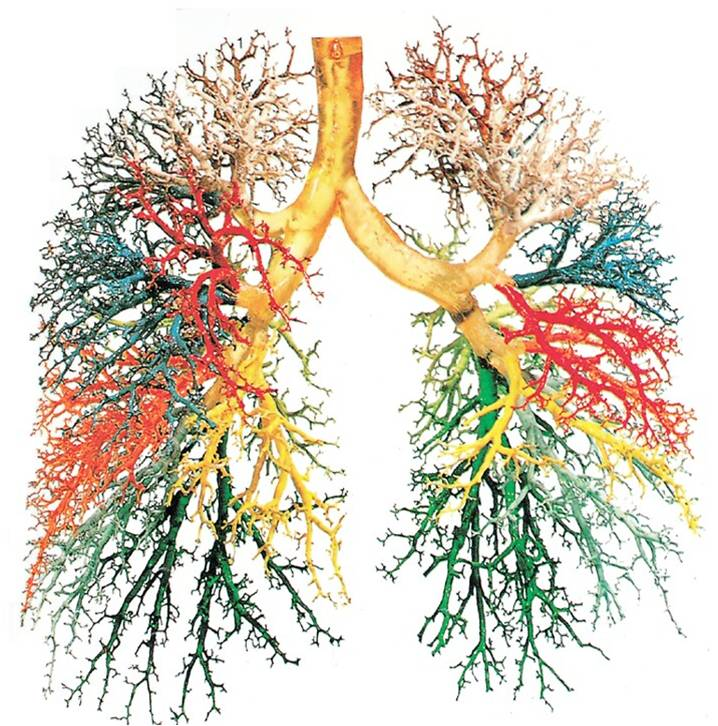
\includegraphics[height=4.7cm]{Images/bronchial-tree.jpg}}
\institute{San Diego State University\\ Applied Mathematics}
\date{December 5, 2019}

\begin{document}
\AtBeginSection{}

    \begin{frame}
        \maketitle
    \end{frame}
    
    \section[Intro]{Introduction}
    
        \begin{frame}{Motivation}
        
            \vfill
            
            \textbf{Goal}: Run implementations for my thesis in my pajamas
            \vfill
            
            \textbf{Problem}: Takes several hours for a complete 10 second debug mode implementation on my laptop
            \vfill
            
            \textbf{Solution}: Optimize time-stepping and linear solver process
            \vfill
        \end{frame}
    
        \begin{frame}{Thesis Background: Biology}
        
            \begin{figure}
                    \centering
                    
                    \subfloat[Branching at the pseudoglandular stage]{\reflectbox{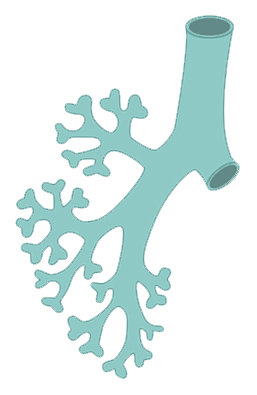
\includegraphics[width=3cm, height=4cm,frame]{Images/lungs2.png}}}\qquad
                    \subfloat[Gene proteins diffuse from lung surface]{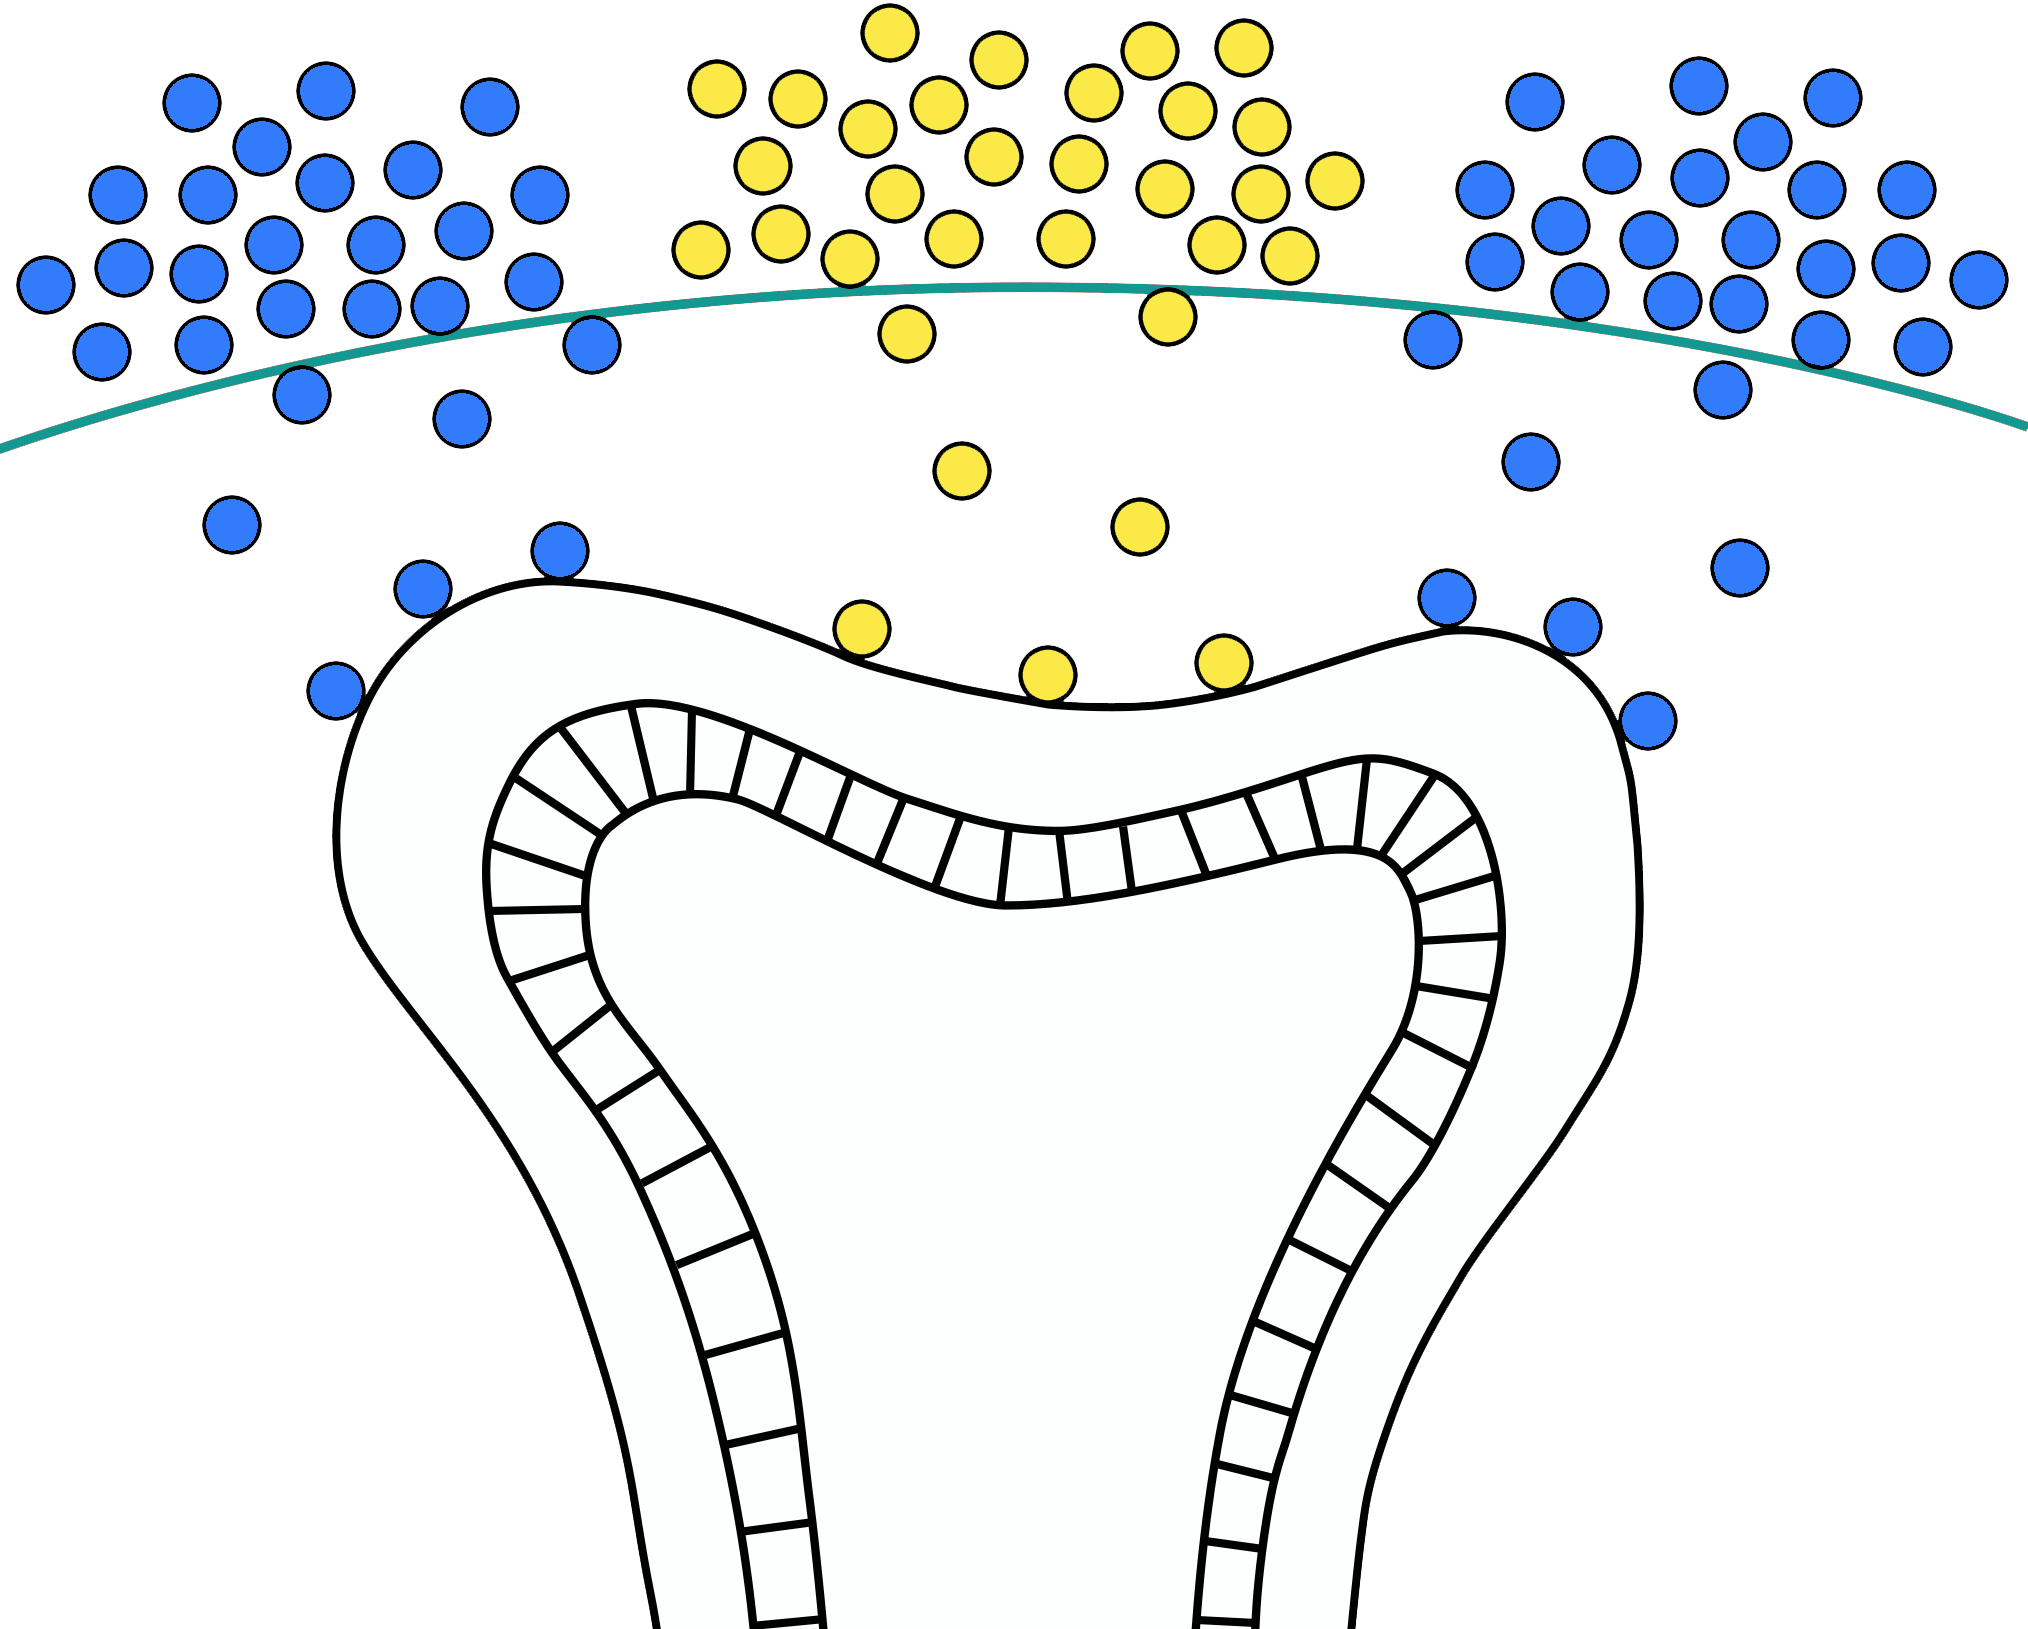
\includegraphics[width=3cm, height=4cm,frame]{Images/lungs_diffusion2.png}}\qquad 
                    \subfloat[Feedback loop between FGF10 and SHH genes]{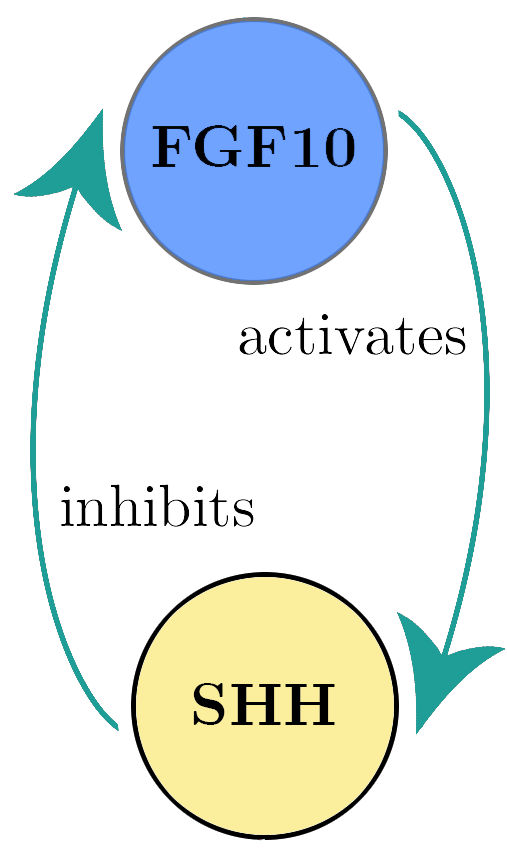
\includegraphics[width=3cm, height=4cm,frame]{Images/feedback_loop2.png}}
                    
                \end{figure}
            
            \end{frame}
    
        \begin{frame}{Thesis Background: Theory}
         


            \begin{center}
                    {\large Auto-catalytic Reaction Model}\\
                    \vspace{-5mm}
                    
                    \begin{large}
                    $$ \ce{X <=>[k_1][k_2] F} ~~~~~~~~~~ \ce{2F + S ->[k_3] 3F} ~~~~~~~~~~ \ce{Y ->[k_4] S} $$
                    \end{large}
                    
                    \vspace{-5mm}
                    {\Huge \textbf{+}} \\
                    
                    {\large Laplace-Beltrami Operator}\\
                    \vspace{-5mm}
                    
                    \begin{equation*}
                        \label{Laplace-Beltrami}
                        \Delta_\Gamma u = \nabla_\Gamma\cdot\nabla_\Gamma u ~~~~~ \text{with} ~~~~~ \nabla_\Gamma u = \nabla u-(\nabla u\cdot\vec{n})\vec{n}
                    \end{equation*}
                    \vspace{-5mm}
                    
                    {\Huge \textbf{=}} \\
                    
                    
                    {\large Schnakenberg Equations on Surface}\\
                    \vspace{-5mm}
                    
                    \begin{equation*}
                        \begin{aligned}
                            & \dot{F} = \nabla^2_\Gamma u + 
                            \gamma\left(\alpha - F + F^2S\right)\\
                            & \dot{S} = \delta\nabla^2_\Gamma S + 
                            \gamma\left(\beta - F^2S\right)\\
                        \end{aligned}
                    \end{equation*}
                    
                \end{center}
            
        \end{frame}
        
            

        
        \begin{frame}{Euler-Midpoint First/Second Order Method}
            
            First, time-step efficiently!
            
            \begin{align*}
                F^{(1)}&=u_{n}+\Delta t~ f\left(u_{n}, v_{n}\right)\\
                F^{(2)}&=u_{n}+\Delta t~ f\left(u_{n}+\frac{1}{2} \Delta t F^{(1)}, v_{n}+\frac{1}{2} \Delta t G^{(1)}\right) 
            \end{align*}
            \vfill
            
            $$\text{With}$$
            
            \vfill
            
            $$e_{n}=\left|F^{(2)}-F^{(1)}\right|, ~~~~~~ \tau = 10^{-3},$$
            $$\chi=\left(\frac{\tau}{\operatorname{norm}\left(e_{n}\right)}\right)^{1/4}, ~~~~~~ \Delta t_{n+1} = \chi\Delta t_n$$
            
            \vfill
            
        \end{frame}
    
    
        \section[Linear System]{The Finite Element Method}    
        
            \begin{frame}{Spatial Discretization}
            
                {\Large $$\dot{F} - \Delta_\Gamma F=                    \gamma\left(\alpha - F + F^2S\right)$$}
                
                
                
                \begin{columns}
                    \column{0.3\textwidth}
                        Multiply by test function, integrate:
                    \column{0.7\textwidth}
                        $$ \int_\Omega\varphi_i(\dot{F}-\Delta_\Gamma F)=
                        \gamma\int_\Omega \frac{}{}\hspace{-2mm} \varphi_i\left(\alpha - F + F^2S\right) $$
                \end{columns}
                
                
                \vspace{5mm}
                
                \begin{columns}
                    \column{0.3\textwidth}
                        Integrate Laplacian term by parts:
                    \column{0.7\textwidth}
                        $$ \int_\Omega \varphi_i \Delta_\Gamma F = \int_{\partial\Omega} \varphi_i\textbf{n} \cdot \nabla F - \int_\Omega \nabla\varphi_i \cdot \nabla F $$
                \end{columns}
                
                
                \vspace{5mm}
                
                \begin{columns}
                    \column{0.3\textwidth}
                        Discretize in space:
                    \column{0.7\textwidth}
                        $$ F \approx \sum_j \varphi_j ~f ~~ \longrightarrow ~~ \int_\Omega \varphi_i F \approx \sum_j(\varphi_i, \varphi_j ~f) $$
                \end{columns}

                
            \end{frame}
            
            
            
            
            
            \begin{frame}{Linear System}
            
                
                {\Large $$\dot{F} - \Delta_\Gamma F= \gamma\left(\alpha - F + F^2S\right)$$}
                
                \vfill
                
                {\large $$\sum_j(\varphi_i, \varphi_j) ~\dot{f} + 
                \sum_j(\nabla\varphi_i, \nabla\varphi_j) ~f = $$
                $$\gamma\left[\alpha\sum_j(\varphi_i, 1) - 
                \sum_j(\varphi_i, \varphi_j) ~f + 
                \sum_j(\varphi_i, \varphi_j) ~f^2s\right]$$}
                
                \vfill 
                
                $$\textbf{M} = \sum(\varphi_i, \varphi_j) ~~~\textbf{A}=\sum(\nabla\varphi_i, \nabla\varphi_j) ~~~ \textbf{C}=\sum(\varphi_i, 1)$$
                
                \vfill
                
            \end{frame}
            
            
            
            
            
            
            \begin{frame}{Time Discretization}
            
            \vspace{-1cm}
                
                {\Large $$\textbf{M}\dot{f} + \textbf{A}f = \gamma\left[\alpha\textbf{C} - \textbf{M}f + \textbf{M}f^2s\right]$$}
                
                 
                
                \vspace{0mm}
                
                \begin{columns}
                
                    \column{0.25\textwidth}
                        
                        IMEX scheme, first order backward Euler:
                        
                    \column{0.75\textwidth}
                    
                        $$ \frac{\textbf{M}(f_{n+1} - f_{n})}{\Delta t} + \textbf{A}f_{n+1} = \gamma\left(\alpha\textbf{C} - \textbf{M}f_{n+1} + \textbf{M}f_{n}^2s_{n}\right) $$

                    
                \end{columns}
                
                 
                
                \begin{columns}
                
                    \column{0.25\textwidth}
                    
                       
                        
                        Solve the linear system Ax=b:
                        
                    \column{0.75\textwidth}
                    
                      
                        
                        $$ \left[\frac{}{}(1+\gamma\Delta t)\textbf{M} + \Delta t \textbf{A}~\right]f_{n+1} = \gamma\Delta t\left(\frac{}{}\alpha\textbf{C} + \textbf{M}f_{n}^2s_{n}\right) $$
                    
                \end{columns}
                
                \vspace{3mm}
                
                We solve the above linear system using the CG method, allowing no more than 10,000 iterations and requiring a convergence tolerance of $10^{-10}$. I neglect a preconditioner.
                
            \end{frame}    


        

        
    

        
    \section[Results]{Results Using the Schnakenberg Equations}
    
        \begin{frame}{Comparison: Convergence (Release Mode)}
        
            \begin{columns}
            
            \column{0.5\textwidth}
            \vspace{-.2cm}
            \begin{figure}
                \centering
                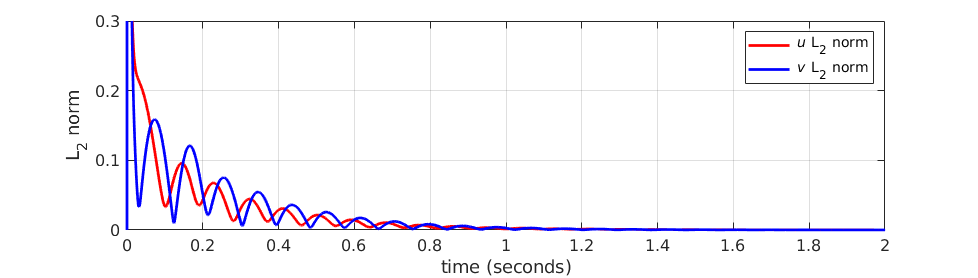
\includegraphics[width = \textwidth, trim={1cm 0cm 1cm 0cm},clip]{Images/none.png}
                \caption*{No adaptive time stepping, deal.ii's CG method: 76 seconds}
                \label{fig:my_label}
            \end{figure}
            
            \vspace{-.2cm}
            
            \begin{figure}
                \centering
                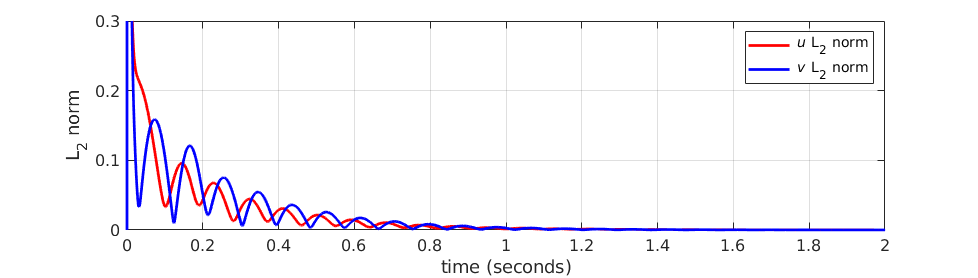
\includegraphics[width = \textwidth, trim={1cm 0cm 1cm 0cm},clip]{Images/none.png}
                \caption*{No adaptive time stepping, my CG method: 45 seconds (no error)}
                \label{fig:my_label}
            \end{figure}
            
            \column{0.5\textwidth}
            \vspace{-.2cm}
            
            \begin{figure}
                \centering
                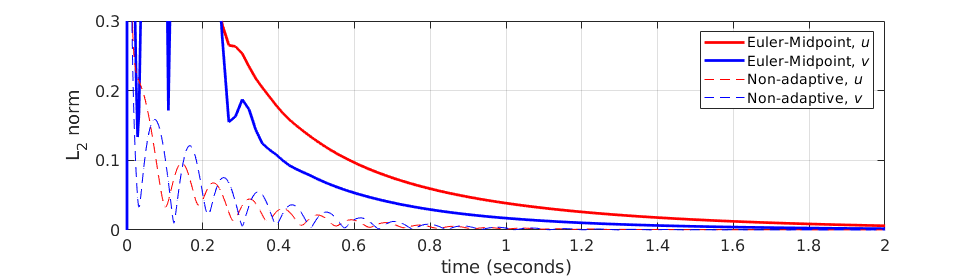
\includegraphics[width = \textwidth, trim={1cm 0cm 1cm 0cm},clip]{Images/euler.png}
                \caption*{Euler time stepping, deal.ii's CG method: 582 steps, 12 seconds}
                \label{fig:my_label}
            \end{figure}
            
             \vspace{-.2cm}
            
            \begin{figure}
                \centering
                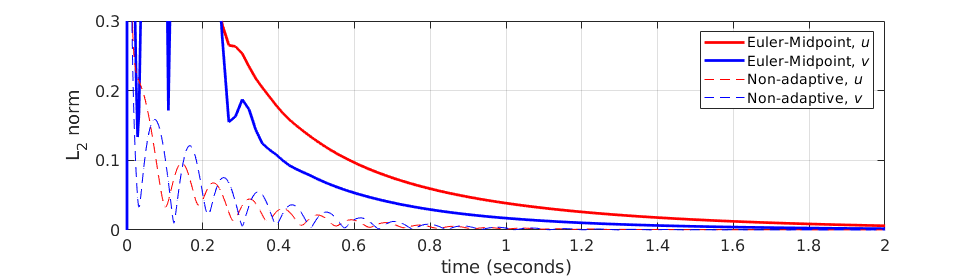
\includegraphics[width = \textwidth, trim={1cm 0cm 1cm 0cm},clip]{Images/euler.png}
                \caption*{Euler time stepping, my CG method: 253 steps, 1 second! (error: $10^{-9}$)}
                \label{fig:my_label}
            \end{figure}
                
            
            \end{columns}
                
            
        \end{frame}
    
    \section[Conclusion]{Conclusions and Next Steps}
    
        \begin{frame}{Conclusions}
        
            Is the preconditioner useless for this problem? \\ Why does my method differ in time steps? \\My CG method using Euler adaptive time steps is the most time efficient, with an acceptable error of $10^{-9}$ Next steps are:
            
            \vfill
            
            \begin{columns}
            
            \column{0.5\textwidth}
                \begin{figure}
                        \centering
                        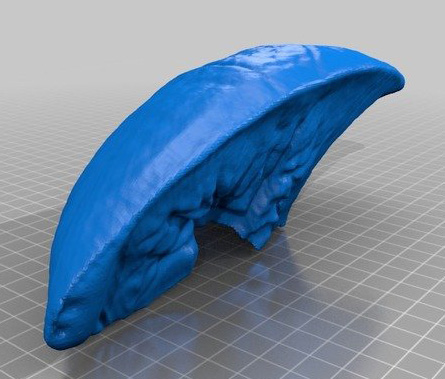
\includegraphics[width = 5cm, frame]{Images/v2lung03.jpg}
                        \caption*{3D model of left lung}
                    \end{figure}
            
            \column{0.5\textwidth}
                \begin{itemize}
                \item Use second order temporal discretization scheme for FEM
                \item Examine model on the mesh of a human lung
                \item Solve on growing domain of developing lung 
                \end{itemize}
            
            \end{columns}
            \vfill
            
        \end{frame}
    
    
    
    
    
    
    
    
    
    
    
    
    
    
    
    
            \appendix
            
            \begin{frame}{Further Reading}
                \nocite{*}
                \bibliography{demo_bibliography}
                \bibliographystyle{ieeetr}
            \end{frame}
    
            \begin{frame}[focus]
                \huge Thank You!\\
            \end{frame}
    
\end{document}

        
        \begin{frame}{Algorithm (general form)}
        
        \begin{align*}
            & \kappa_{1u} = \Delta t ~ \gamma ~ (\alpha\textbf{F} - \textbf{M}U + \textbf{M}U^2V) \\
            & \kappa_{1v} = \Delta t ~ \gamma ~(\beta\textbf{F} - \textbf{M}U^2V) \\
            & ... \\
            & \text{plug $\kappa$'s into $F^{(n)}$ and $F^{(m)}$} \\
            & \text{find absolute value of difference $\left|F^{(n)} - F^{(n)}\right|$} \\
            & \chi=\left(\frac{\tau}{\operatorname{norm}\left(\text{difference}\right)}\right)^{1/4}\\
            & \Delta t = \chi\cdot\Delta t\\
        \end{align*}
            
        \end{frame}

    
    \section[Introduction]{Introduction, Background, and Research Motivation}
            
            \begin{frame}{The Developing Lung}
            
                \begin{columns}
                
                \column{0.4\textwidth}
                    \begin{figure}
                        \centering
                        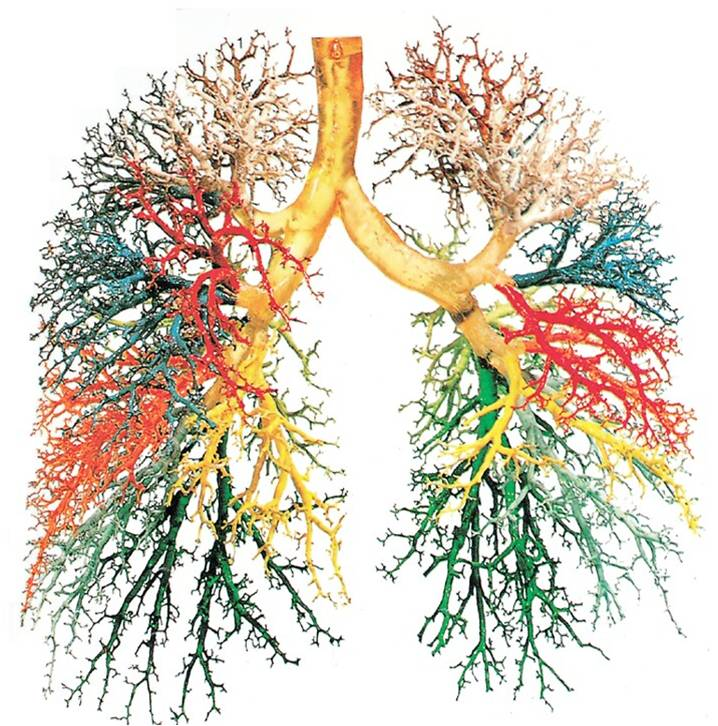
\includegraphics[width = 5cm, frame]{Images/bronchial-tree.jpg}
                        \caption*{Visualization of adult lung branching structures}
                        \label{fig:my_label}
                    \end{figure}
                    
                     
                    
                \column{0.4\textwidth}
                \vspace{-1cm}
                    \begin{itemize}
                        \item Introduction on Lung branching mechanics and the equations that may describe their behavior
                         \item Examining Turing instability regions analytically
                         \item Translating system to finite elements
                    \end{itemize}
                
                \end{columns}
                
            \end{frame}
    
           
            \begin{frame}{Branching Morphogenesis}

                \begin{figure}
                    \centering
                    
                    \subfloat[Branching at the pseudoglandular stage]{\reflectbox{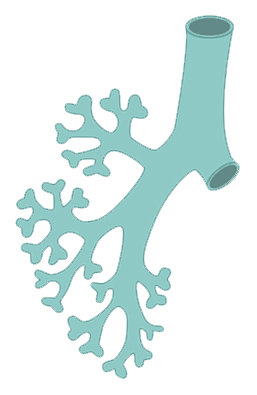
\includegraphics[width=3cm, height=4cm,frame]{Images/lungs2.png}}}\qquad 
                     
                    \subfloat[Gene proteins diffuse from lung surface]{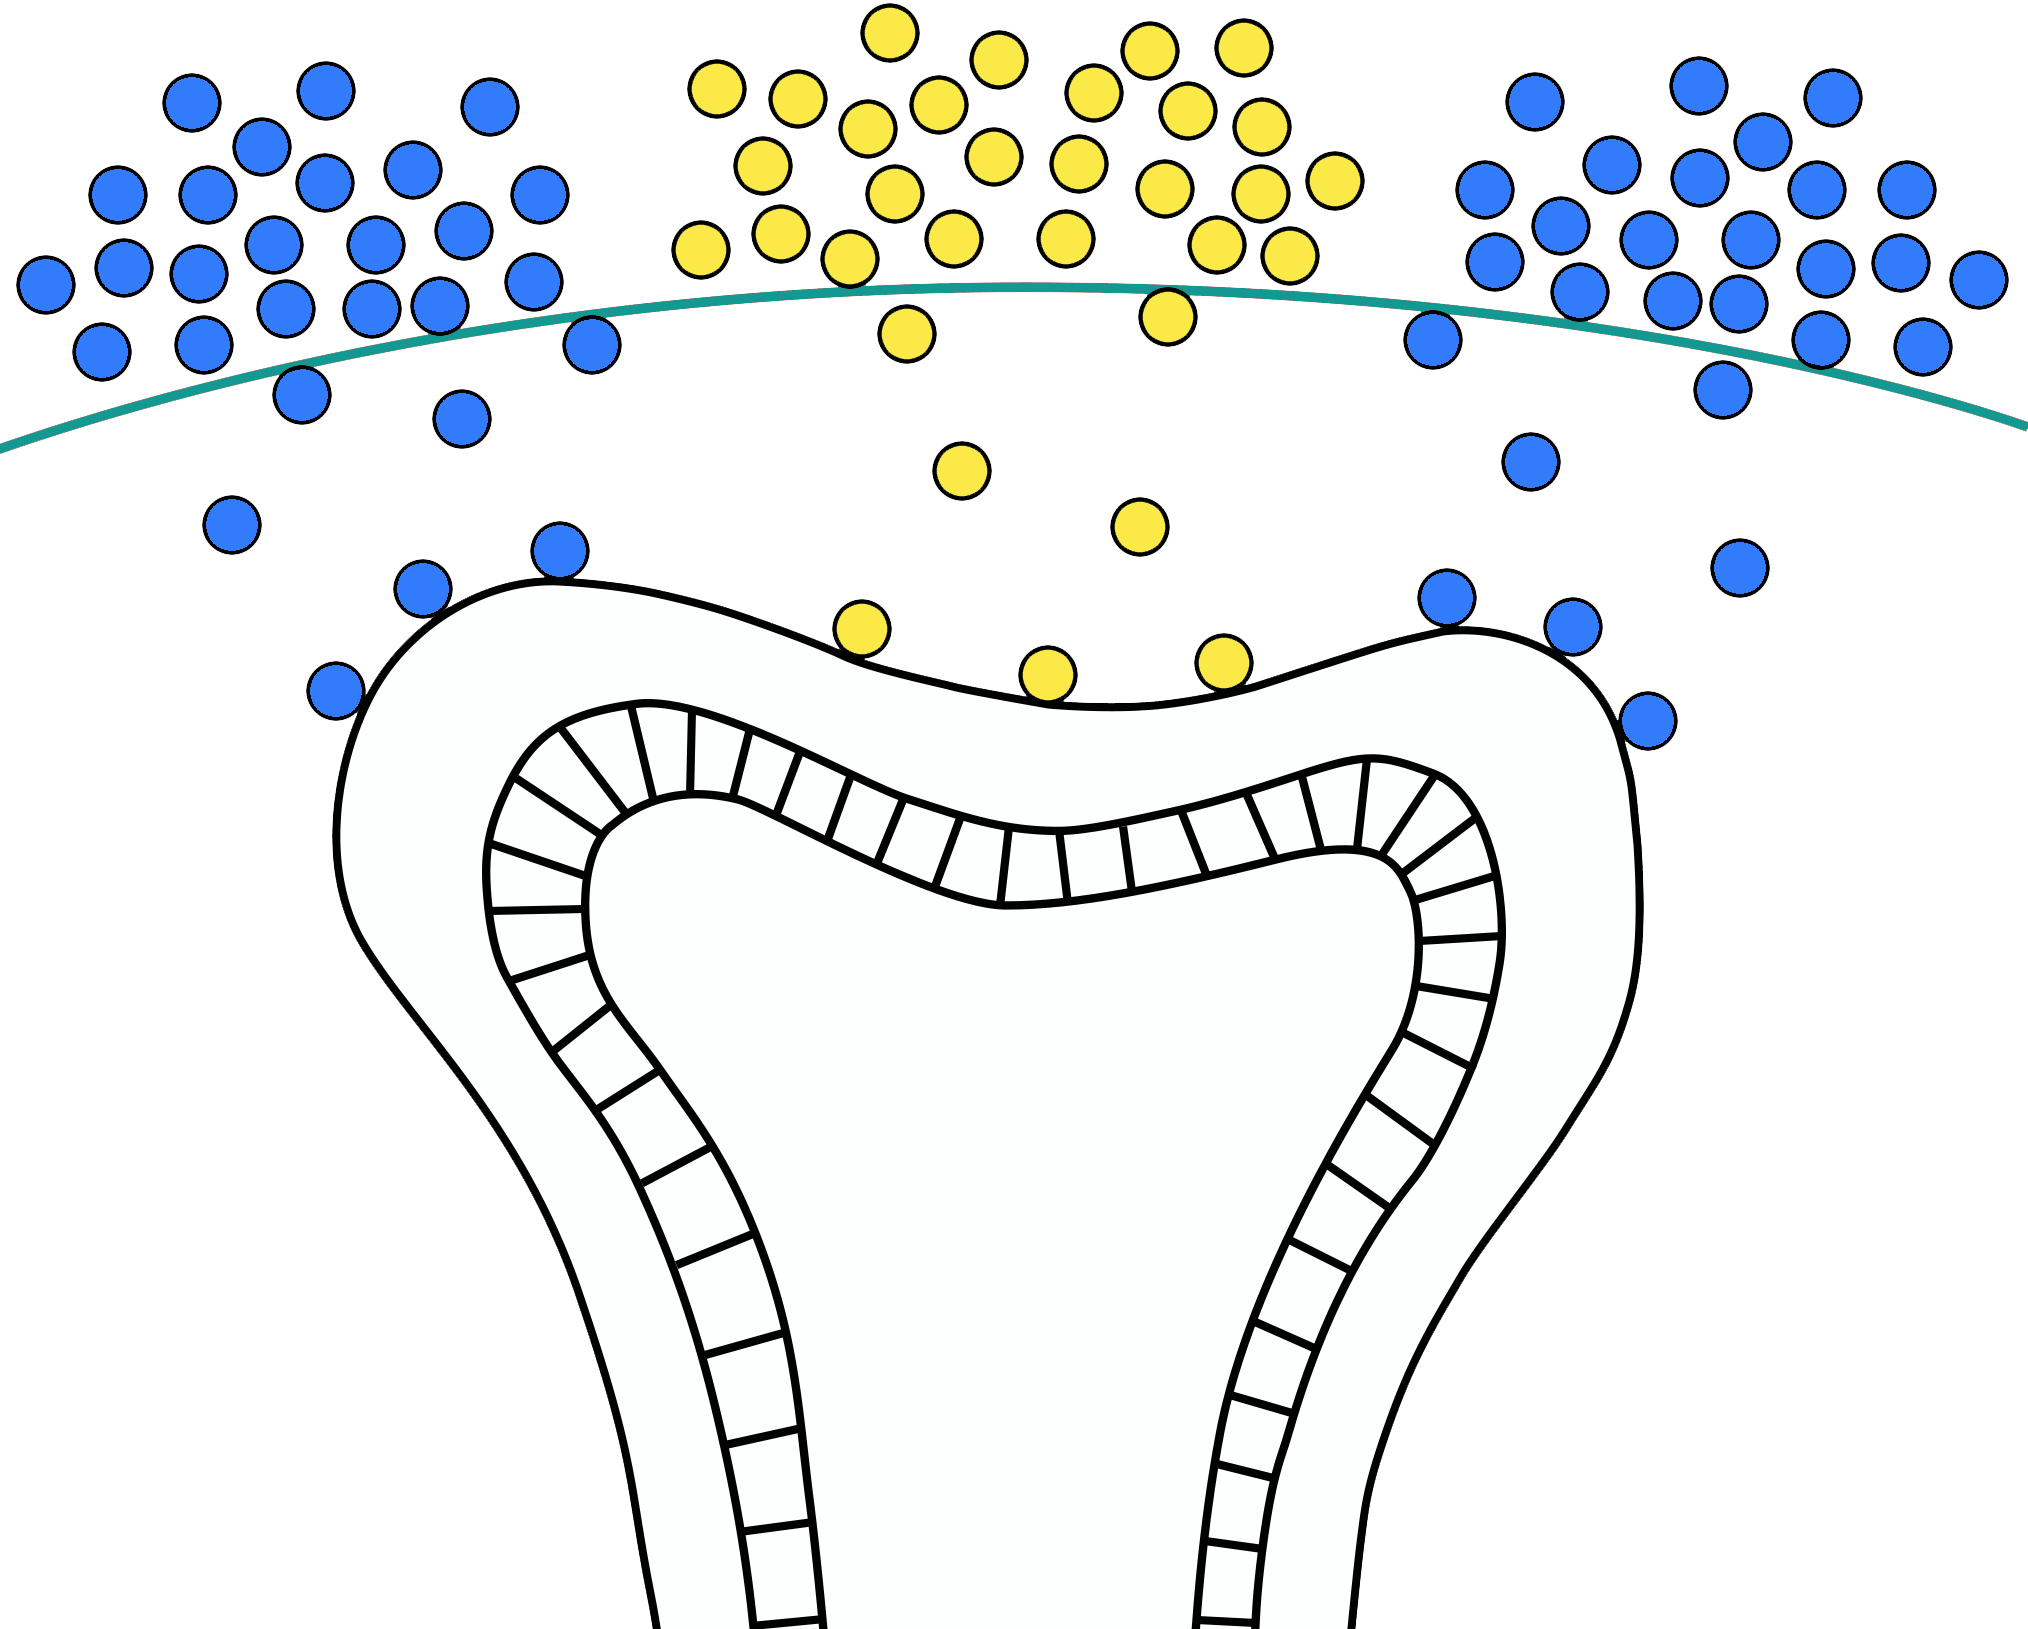
\includegraphics[width=3cm, height=4cm,frame]{Images/lungs_diffusion2.png}}\qquad
                     
                    \subfloat[Feedback loop between FGF10 and SHH genes]{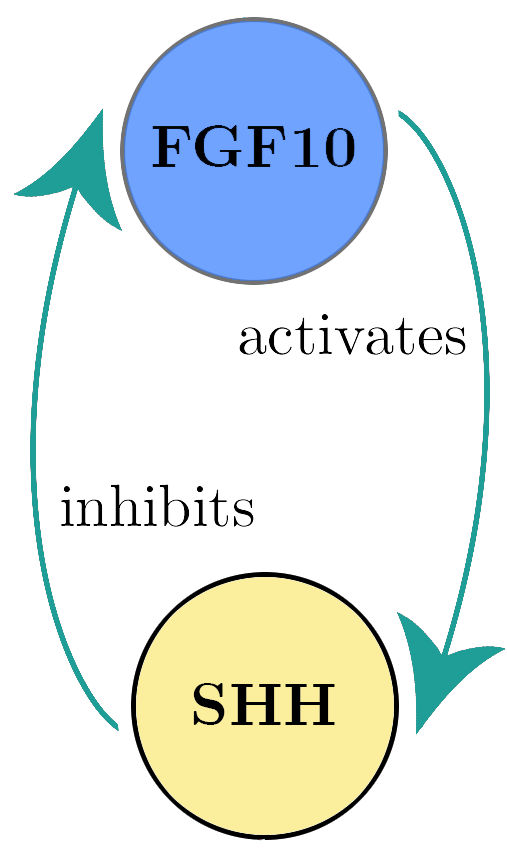
\includegraphics[width=3cm, height=4cm,frame]{Images/feedback_loop2.png}}
                    
                \end{figure}
            
            \end{frame}
            
            \begin{frame}{Research Motivation}
            
                \begin{columns}
                    \column{0.55\textwidth}
                        \textbf{Applications to lung regeneration and disease research:} \\
                         \vspace{5mm}
                        Congenital Diaphragmatic Hernias (CDH) causes hypoplastic lung development in the fetus. There is currently no treatment to encourage continued branching growth postpartum.
                    \column{0.45\textwidth}
                        \begin{figure}
                            \centering
                            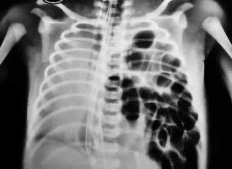
\includegraphics[width=5cm, frame]{Images/v2lung02.jpg}
                            \caption*{Left-sided CDH in infant}
                        \end{figure}
                \end{columns}
            
            \end{frame}
            
            
            
            \begin{frame}{Turing's Theory}
            
                \begin{columns}
                
                \column{0.4\textwidth}
                
                    \begin{figure}
                        \centering
                        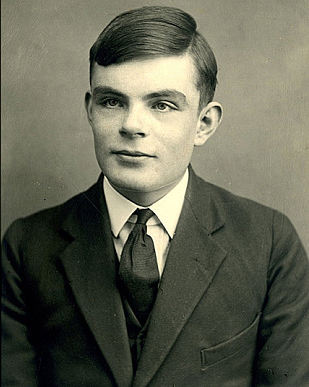
\includegraphics[width = 4cm]{Images/turing.jpg}
                        \caption*{Alan Turing, 1928}
                        \label{fig:my_label}
                    \end{figure}
                    
                 
                
                \column{0.5\textwidth}
                
                    \begin{itemize}
                        \item Groundbreaking 1952 paper \textit{The Chemical Basis of Morphogenesis} \vfill
                        \item Homogeneous, stable systems may become unstable with the addition of diffusion \vfill
                        \item \textit{Turing Instability} may give rise to biological patterns
                    \end{itemize}
                    
                \end{columns}
            
                
                
                
                
            \end{frame}
            
        
            \begin{frame}{Model Equations}
            
                \begin{center}
                    {\large Auto-catalytic Reaction Model}\\
                    \vspace{-5mm}
                    
                    \begin{large}
                    $$ \ce{X <=>[k_1][k_2] F} ~~~~~~~~~~ \ce{2F + S ->[k_3] 3F} ~~~~~~~~~~ \ce{Y ->[k_4] S} $$
                    \end{large}

                    
                    \vspace{-5mm}
                     
                    {\Huge \textbf{+}} \\
                    
                    
                    {\large Laplace-Beltrami Operator}\\
                    \vspace{-5mm}
                    
                    \begin{equation*}
                        \label{Laplace-Beltrami}
                        \Delta_\Gamma u = \nabla_\Gamma\cdot\nabla_\Gamma u ~~~~~ \text{with} ~~~~~ \nabla_\Gamma u = \nabla u-(\nabla u\cdot\vec{n})\vec{n}
                    \end{equation*}
                    \vspace{-5mm}
                    
                    
                     
                    {\Huge \textbf{=}} \\
                    
                    
                    {\large Schnakenberg Equations on Surface}\\
                    \vspace{-5mm}
                    
                    \begin{equation*}
                        \begin{aligned}
                            & \dot{F} = \Delta_\Gamma F + 
                            \gamma\left(\alpha - F + F^2S\right)\\
                            & \dot{S} = \delta\Delta_\Gamma S + 
                            \gamma\left(\beta - F^2S\right)\\
                        \end{aligned}
                    \end{equation*}
                    

                
                \end{center}
            
            \end{frame}
            
            
            
            
        
    \section[Turing Regions]{Turing Instability Regions}
        
            \begin{frame}{Stability Without Diffusion}

                

                \begin{equation*}
                        \left.\begin{aligned}
                            & \dot{F} = 
                            \gamma\left(\alpha - F + F^2S\right)\\
                            & \dot{S} =  
                            \gamma\left(\beta - F^2S\right)\\
                        \end{aligned}\right\} ~~~~~
                        \xrightarrow[]{\text{~~Taylor Expansion~~}}~~~~~ \dot{W}=\gamma~J_*W
                    \end{equation*} 
                    
                \begin{multicols}{2}[]
                
                 

                ~ \\
                
                \center{Equilibrium point: ~~~ $ \left(\alpha+\beta,\frac{\beta}{(\alpha+\beta)^2}\right) $
                
                \vfill
                
                Stable parameters: ~~~ $ \beta-\alpha < (\alpha+\beta)^3 $}
                
                \vfill
                
                \columnbreak
                
                \begin{figure}[H]
                    \centering
                    \subfloat
                    [Stability region for $\alpha$ and $\beta$]{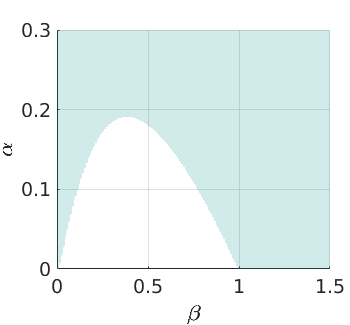
\includegraphics[width = 4.5cm]{Images/param_0.png}}
                \end{figure}
                
                \end{multicols}
                
                
                

            \end{frame}
            

        
            \begin{frame}{Analytic Solution}
            
                \begin{center}
                
                \begin{equation*}
                        \left.\begin{aligned}
                            & \dot{F} = \Delta_\Gamma F +
                            \gamma\left(\alpha - F + F^2S\right)\\
                            & \dot{S} =  \delta\Delta_\Gamma S +
                            \gamma\left(\beta - F^2S\right)\\
                        \end{aligned}\right\} ~~~~~\xrightarrow[]{\text{~~~~~~}}~~~~~ \dot{W}=D\Delta_\Gamma W+\gamma~J_*W
                    \end{equation*}
                    
                     

                \vspace{3mm}
                
                {\large Eigenvalue Problem:  ~~~~~$ \dot{W}=\lambda W ~~~~~\text{and}~~~~~ \Delta_\Gamma W = -k^2W $}

                 
                
                \vspace{-3mm}
                
                {\Large
                $$W(\phi,\theta,t)=\sum_{m=0}^\infty \sum_{n \geq m}^{\infty} A_{mn}\cdot e^{\lambda t}\cdot Y_n^m(\phi,\theta)$$}
                
                \vspace{-2mm}
                
                {
                $$\text{with ~~~~~ }A_{mn} = \frac{\int_0^\pi\int_{-\pi}^\pi W_*Y_n^m(\phi,\theta)\sin{\phi}d\theta d\phi}{\int_0^\pi\int_{-\pi}^\pi [Y_n^m(\phi,\theta)]^2\sin{\phi}d\theta d\phi}$$}
                
                \end{center}
            
            \end{frame}
            
            
            \begin{frame}{Instability with Diffusion}
                \vspace{-3mm}
                {\Large $$ \lambda W = -k^2W +\gamma~J_*W ~~~~~\longrightarrow~~~~~ \det(  - Dk^2 + \gamma~J-\lambda I ) = 0 $$} 
                \vspace{-3mm}
                 
                
                \begin{columns}
                    
                    \column{0.24\textwidth}
                        {\small $$ \text{~~~~~}\delta(\beta-\alpha) > (\alpha+\beta)^3 $$}
                    \column{0.52\textwidth}
                        ~
                \end{columns}
                
                \vspace{-3mm}
                
                \begin{figure}[H]
                    \centering
                    \subfloat
                    [Delta regions for $\alpha$ and $\beta$ constraints to induce instability]{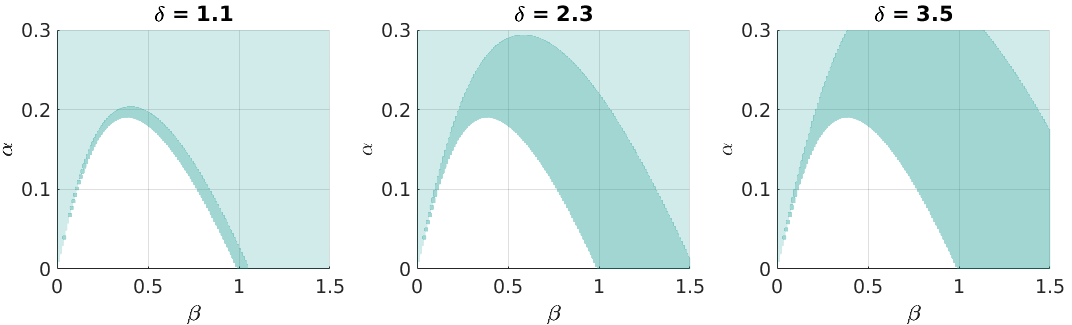
\includegraphics[width = 10.5cm]{Images/param_1_green.png}}
                \end{figure}
            \end{frame}
            
            
            
            
            \begin{frame}{Instability with Diffusion}
                \vspace{-3mm}
                {\Large $$ \lambda W = -k^2W +\gamma~J_*W ~~~~~\longrightarrow~~~~~ \det(  - Dk^2 + \gamma~J-\lambda I ) = 0 $$} 
                \vspace{-3mm}
                
                \begin{columns}
                    
                    \column{0.24\textwidth}
                        {\small $$ \text{~~~~~}\delta(\beta-\alpha) > (\alpha+\beta)^3 $$}
                    \column{0.52\textwidth}
                        {\small $$ \text{~~~~} \left(\frac{}{}\delta(\beta-\alpha)-(\alpha+\beta)^3\right)^2 > 4\delta(\alpha+\beta)^4 $$}
                \end{columns}
                
                \vspace{-3mm}
                
                \begin{figure}[H]
                    \centering
                    \subfloat
                    [Delta regions for $\alpha$ and $\beta$ constraints to induce instability]{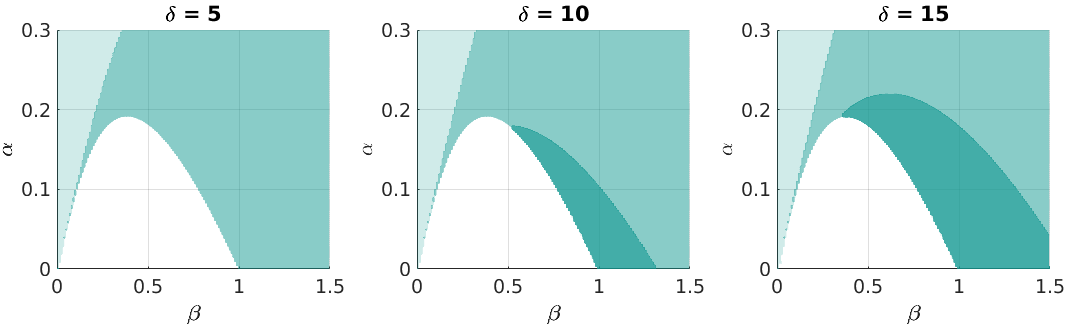
\includegraphics[width = 10.5cm]{Images/param_2.png}}
                \end{figure}
            \end{frame}
            
            
            \begin{frame}{Eigenvalue Solutions}
            
               
                \begin{center}
                    {\Large Isolate single $n$ such that $k^2_- < k^2_c = n(n+1) < k^2_+$}
                \end{center}
                
                
                $$
                k^2 = \frac{\delta(\beta-\alpha) - (\alpha+\beta)^3 \pm \sqrt{[\delta(\beta-\alpha) - (\alpha+\beta)^3]^2 - 4\delta(\alpha+\beta)^4}}{2\delta(\alpha+\beta)}
                $$
                
                 
            
                \begin{figure}
                    \centering
                    \subfloat[n = 2]{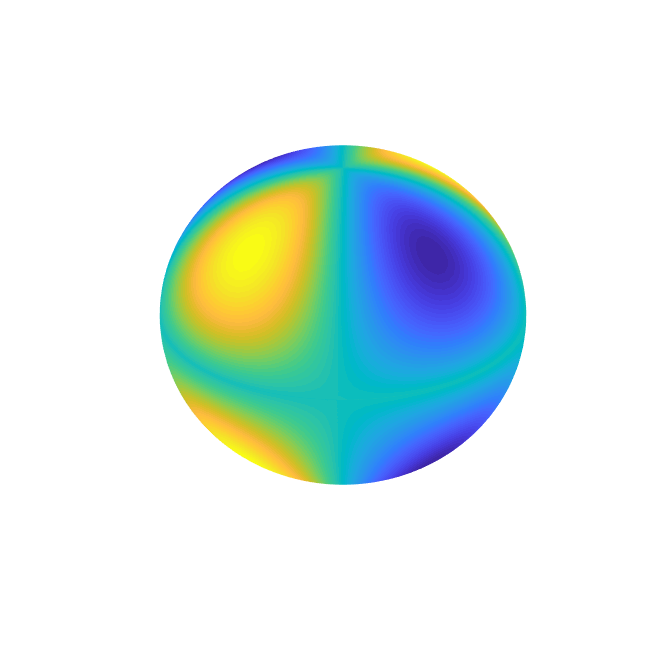
\includegraphics[width=3cm, trim={3cm 3cm 3cm 3cm},clip]{Images/sphere_2.png}}\qquad % 
                    \subfloat[n = 4]{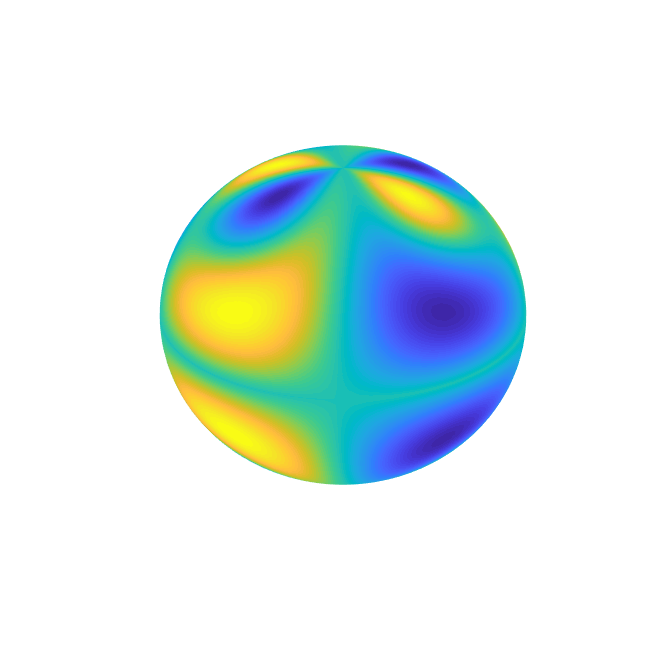
\includegraphics[width=3cm, trim={3cm 3cm 3cm 3cm},clip]{Images/sphere_4.png}}\qquad % 
                    \subfloat[n = 20]{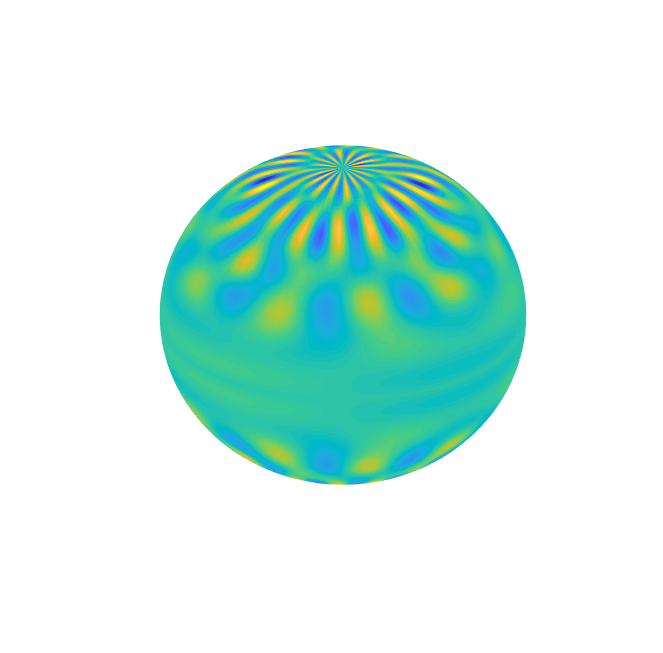
\includegraphics[width=3cm, trim={3cm 3cm 3cm 3cm},clip]{Images/sphere_20.png}}
                    
                \end{figure}
            \end{frame}
            
            
            
            
            

            
            
            
            
            
            
            
            
        \section[Finite Elements]{The Finite Element Method}    
        
            \begin{frame}{Spatial Discretization}
            
                {\Large $$\dot{F} - \Delta_\Gamma F=                    \gamma\left(\alpha - F + F^2S\right)$$}
                
                
                
                \begin{columns}
                    \column{0.3\textwidth}
                        Multiply by test function, integrate:
                    \column{0.7\textwidth}
                        $$ \int_\Omega\varphi_i(\dot{F}-\Delta_\Gamma F)=
                        \gamma\int_\Omega \frac{}{}\hspace{-2mm} \varphi_i\left(\alpha - F + F^2S\right) $$
                \end{columns}
                
                
                \vspace{5mm}
                
                \begin{columns}
                    \column{0.3\textwidth}
                        Integrate Laplacian term by parts:
                    \column{0.7\textwidth}
                        $$ \int_\Omega \varphi_i \Delta_\Gamma F = \int_{\partial\Omega} \varphi_i\textbf{n} \cdot \nabla F - \int_\Omega \nabla\varphi_i \cdot \nabla F $$
                \end{columns}
                
                
                \vspace{5mm}
                
                \begin{columns}
                    \column{0.3\textwidth}
                        Discretize in space:
                    \column{0.7\textwidth}
                        $$ F \approx \sum_j \varphi_j ~f ~~ \longrightarrow ~~ \int_\Omega \varphi_i F \approx \sum_j(\varphi_i, \varphi_j ~f) $$
                \end{columns}

                
            \end{frame}
            
            
            
            
            
            \begin{frame}{Linear System}
            
                
                {\Large $$\dot{F} - \Delta_\Gamma F= \gamma\left(\alpha - F + F^2S\right)$$}
                
                \vfill
                
                {\large $$\sum_j(\varphi_i, \varphi_j) ~\dot{f} + 
                \sum_j(\nabla\varphi_i, \nabla\varphi_j) ~f = $$
                $$\gamma\left[\alpha\sum_j(\varphi_i, 1) - 
                \sum_j(\varphi_i, \varphi_j) ~f + 
                \sum_j(\varphi_i, \varphi_j) ~f^2s\right]$$}
                
                \vfill 
                
                $$\textbf{M} = \sum(\varphi_i, \varphi_j) ~~~\textbf{A}=\sum(\nabla\varphi_i, \nabla\varphi_j) ~~~ \textbf{C}=\sum(\varphi_i, 1)$$
                
                \vfill
                
            \end{frame}
            
            
            
            
            
            
            \begin{frame}{Time Discretization}
            
            \vspace{-1cm}
                
                {\Large $$\textbf{M}\dot{f} + \textbf{A}f = \gamma\left[\alpha\textbf{C} - \textbf{M}f + \textbf{M}f^2s\right]$$}
                
                 
                
                \vspace{0mm}
                
                \begin{columns}
                
                    \column{0.25\textwidth}
                        
                        IMEX scheme, first order backward Euler:
                        
                    \column{0.75\textwidth}
                    
                        $$ \frac{\textbf{M}(f_{n+1} - f_{n})}{\Delta t} + \textbf{A}f_{n+1} = \gamma\left(\alpha\textbf{C} - \textbf{M}f_{n+1} + \textbf{M}f_{n}^2s_{n}\right) $$

                    
                \end{columns}
                
                 
                
                \begin{columns}
                
                    \column{0.25\textwidth}
                    
                       
                        
                        Solve the linear system Ax=b:
                        
                    \column{0.75\textwidth}
                    
                      
                        
                        $$ \left[\frac{}{}(1+\gamma\Delta t)\textbf{M} + \Delta t \textbf{A}~\right]f_{n+1} = \gamma\Delta t\left(\frac{}{}\alpha\textbf{C} + \textbf{M}f_{n}^2s_{n}\right) $$
                    
                \end{columns}
                
            \end{frame}    
            
            
            
            
            \begin{frame}{Solving Numerically}
            
                \begin{columns}
                
                    \column{0.45\textwidth}
                    
                        \begin{itemize}
                            \item The conjugate gradient iterative method was used to solve the linear system.
                            \item The finite element code was implemented using the C++ library \textit{deal.ii}
                            
                        \end{itemize}
                        
                        
                    \column{0.55\textwidth}
                        \begin{figure}
                            
\includegraphics[width = 6cm, frame]{Images/logo_dealii.png}
                            \label{fig:my_label}
                        \end{figure}
                    
                \end{columns}
            
                

                

                
            \end{frame}
            
            
            
            
            
            
            
            
            
            
            
            
            
            
        


        
    \section[Future Work]{Next Steps and Future Work}
        
            \begin{frame}{Future Work}
            
                \vfill
            
                \begin{columns}
                
                \column{0.4\textwidth}
                    \begin{figure}
                            \centering
                            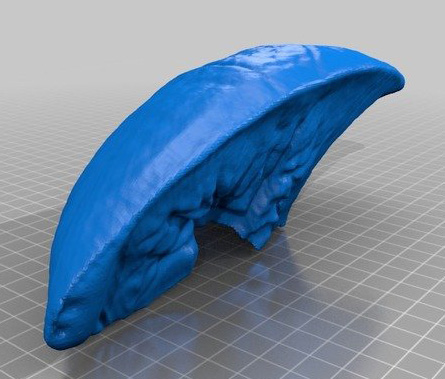
\includegraphics[width = 5cm, frame]{Images/v2lung03.jpg}
                            \caption*{3D model of left lung}
                        \end{figure}
                    
                
                
                \column{0.6\textwidth}
                    \begin{itemize}
                    \item Use second order temporal discretization scheme: may allow larger time steps 
                    \item Optimize time step length using adaptive algorithm  
                    \item Examine model on the mesh of a human lung  
                    \item Solve on growing domain of developing lung
                    \end{itemize}
                    
                
                \end{columns}
                \vfill
            
            \end{frame}
            
        \begin{frame}{Dormand-Prince Fourth/Fifth Order Method}
        
            \vspace{-3mm}
        
            $$F^{(4)}=y_{n}+\frac{5179}{57600} \kappa_{1}+\frac{7571}{16695} \kappa_{3}+\frac{393}{640} \kappa_{4}-\frac{92097}{339200} \kappa_{5}+\frac{187}{2100} \kappa_{6}+\frac{1}{40} \kappa_{7}$$
            $$F^{(5)}=y_{n}+\frac{35}{384} \kappa_{1}+\frac{500}{1113} \kappa_{3}+\frac{125}{192} \kappa_{4}-\frac{187}{6784} \kappa_{5}+\frac{11}{84} \kappa_{6}$$
            
            \vspace{5mm}
            
            {\tiny
            \begin{align*}
                \kappa_{1}&=\Delta t f\left(u_{n}, t_{n}\right) ~~~~~~~~~~ \kappa_{2}=\Delta t f\left(u_{n}+\frac{1}{5} \kappa_{1}, t_{n}+\frac{1}{5}\Delta t\right)\\
                \kappa_{3}&=\Delta t f\left(u_{n}+\frac{3}{40} \kappa_{1}+\frac{9}{40} \kappa_{2}, t_{n}+\frac{3}{10} \Delta t\right)\\
                \kappa_{4}&=\Delta t f\left(u_{n}+\frac{44}{45} \kappa_{1}-\frac{56}{15} \kappa_{2}+\frac{32}{9} K_{3}, t_{n}+\frac{4}{5} \Delta t\right)\\
                \kappa_{5}&=\Delta t f\left(u_{n}+\frac{19372}{6561} {\kappa}_{1}-\frac{25360}{2187} \kappa_{2}+\frac{64448}{6561} {\kappa}_{3}-\frac{212}{729} \kappa_{4}, t_{n}+\frac{8}{9} \Delta t\right)\\
                \kappa_{6}&=\Delta t f\left(u_{n}+\frac{9017}{3168} \kappa_{1}-\frac{355}{33} \kappa_{2}+\frac{46732}{5247} \kappa_{3}+\frac{49}{176} \kappa_{4}-\frac{5103}{18656} \kappa_{5}, t_{n}+\Delta t\right)\\
                \kappa_{7}&=\Delta t f\left(u_{n}+\frac{35}{384} \kappa_{1}+\frac{500}{1113} \kappa_{3}+\frac{125}{192} \kappa_{4}-\frac{187}{6784} \kappa_{5}+\frac{11}{84} \kappa_{6}, t_{n}+\Delta t\right)
            \end{align*}
            }
            
        \end{frame}

